% Under Creative Commons Attribution licence 3.0
% (http://creativecommons.org/licences/by/3.0)
% Author: Florian Lesaint
\documentclass[dvipdfm]{article}
\usepackage{tikz}
\usetikzlibrary{calc}
\begin{document}
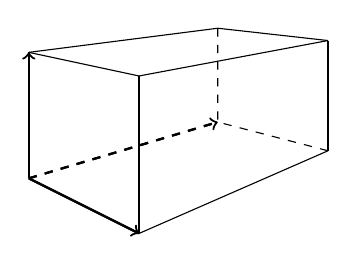
\begin{tikzpicture}
    
	%% 透視投影Vanishing points for perspective handling
	\coordinate (P1) at (-7cm,1.5cm); % left vanishing point (To pick)
	\coordinate (P2) at (8cm,1.5cm); % right vanishing point (To pick)

	%% (A1) and (A2) defines the 2 central points of the cuboid
	\coordinate (A1) at (0em,0cm); % central top point (To pick)
	\coordinate (A2) at (0em,-2cm); % central bottom point (To pick)

	%% (A3) to (A8) are computed given a unique parameter (or 2) .8
	% You can vary .8 from 0 to 1 to change perspective on left side
	\coordinate (A3) at ($(P1)!.8!(A2)$); % To pick for perspective 
	\coordinate (A4) at ($(P1)!.8!(A1)$);

	% You can vary .8 from 0 to 1 to change perspective on right side
	\coordinate (A7) at ($(P2)!.7!(A2)$);
	\coordinate (A8) at ($(P2)!.7!(A1)$);

	%% Automatically compute the last 2 points with intersections
	\coordinate (A5) at
	  (intersection cs: first line={(A8) -- (P1)},
			    second line={(A4) -- (P2)});
	\coordinate (A6) at
	  (intersection cs: first line={(A7) -- (P1)}, 
			    second line={(A3) -- (P2)});

	%%% Depending of what you want to display, you can comment/edit
	%%% the following lines

	%% Possibly draw back faces

	
	\draw[dashed] (A5) -- (A6);
	\draw[thick,dashed] (A3) -- (A6);
	\draw[dashed] (A7) -- (A6);

	%% Possibly draw front faces

	% \fill[orange] (A1) -- (A8) -- (A7) -- (A2) -- cycle; % face 1
	% \node at (barycentric cs:A1=1,A8=1,A7=1,A2=1) {\tiny f1};
	\fill[gray!50,opacity=0.0] (A1) -- (A2) -- (A3) -- (A4) -- cycle; 
	\fill[gray!90,opacity=0.0] (A1) -- (A4) -- (A5) -- (A8) -- cycle; %top
	
	%% 線を描く
	\draw (A1) -- (A2);
	\draw[thick] (A3) -- (A4);
	\draw (A7) -- (A8);
	\draw (A1) -- (A4);
	\draw (A1) -- (A8);
	\draw[thick] (A2) -- (A3);
	\draw (A2) -- (A7);
	\draw (A4) -- (A5);
	\draw (A8) -- (A5);
\draw[->,thick] (A3) -- (A2);
\draw[->,thick] (A3) -- (A4);
\draw[->,thick,dashed] (A3) -- (A6);
 node[right] at(A6) {u};
\end{tikzpicture}
\end{document} 
